%!TEX TS-program = xelatex
\documentclass[]{friggeri-cv}
\usepackage{afterpage}
\usepackage{hyperref}
\usepackage{color}
\usepackage{xcolor}
\hypersetup{
    pdftitle={},
    pdfauthor={},
    pdfsubject={},
    pdfkeywords={},
    colorlinks=false,       % no lik border color
   allbordercolors=white    % white border color for all
}
\addbibresource{bibliography.bib}
\RequirePackage{xcolor}
\definecolor{pblue}{HTML}{0395DE}

\begin{document}
\header{Carlos}{Murillo Badilla}
      {Information Systems Engineer}
      
% Fake text to add separator      
\fcolorbox{white}{gray}{\parbox{\dimexpr\textwidth-2\fboxsep-2\fboxrule}{%
.....
}}

% In the aside, each new line forces a line break
\begin{aside}
  \section{Address}
    Heredia, San Pablo
    ~
  \section{Telephone}% \& Skype}
    \href{tel:87409365}{(+506) 87409365}
    %cmb28@hotmail.com
    ~
  \section{Mail}
    \href{mailto:cmb2897@gmail.com}{cmb2897@gmail.com}
    ~
  \section{Git \& LinkedIn}
    \href{https://github.com/CarlosMurillo2897/}{\textbf{github.com/}\\CarlosMurillo2897}
    ~
    \href{https://www.linkedin.com/in/carlos-mb/}{\textbf{linkedin.com/in/}\\carlos-mb}
    ~
  \section{Programming}
    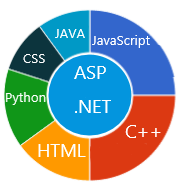
\includegraphics[scale=0.62]{img/Languages.png}
    ~
  \section{OS Preference}
    \textbf{GNU/Linux}
\includegraphics[scale=0.40]{img/5stars.png}
    \textbf{Windows}
\includegraphics[scale=0.40]{img/5stars.png}
    \textbf{MacOS}
\includegraphics[scale=0.40]{img/1stars.png}
    ~
  \section{Databases}
    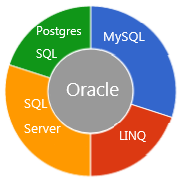
\includegraphics[scale=0.62]{img/DB.png}
    ~
   \section{Languages}
    \textbf{Spanish}
\includegraphics[scale=0.40]{img/5stars.png}
    \textbf{English}
\includegraphics[scale=0.40]{img/4stars.png}
\end{aside}

\section{Education}
\begin{entrylist}
  \entry
    {2015 - 2020}
    {Systems Engineering Bachelor Degree}
    {National University of Costa Rica}
    
  \entry
    {2015 - 2019}
    {Systems Engineering Diploma Degree}
    {National University of Costa Rica}
    
\end{entrylist}

\section{Certifications}
\begin{entrylist}

    \entry
    {2017}
    {CCNA Routing and Switching Module I}
    {National University of Costa Rica}

    \entry
    {2019}
    {SCRUM Fundamentals Certified}
    {SCRUMStudy}
    
    \entry
    {2019}
    {JAVA Basics}
    {National University of Costa Rica}
    
    \entry
    {2020}
    {Learn Perl 5 By Doing It}
    {Udemy}
    
    \entry
    {2020}
    {The Complete Regular Expressions Course 2020}
    {Udemy}
    
    \entry
    {2020}
    {Unlock Excel VBA and Excel Macros}
    {Udemy}
    
    \entry
    {2020}
    {Mastering LINQ with C# and .NET}
    {Udemy}
    
    \entry
    {2020}
    {Ui Path RPA Developer Advanced}
    {UiPath Academy}
    
    \entry
    {2020}
    {Blue Prism Foundation Training}
    {BluePrism University}
    
\end{entrylist}

\section{Further Training}
\begin{entrylist}
    \entry
    {}
    {Programming Knowledge}
    {}
    {C++, Android, JavaScript (Jquery, AJAX, Json), HTML, Python, Nodejs, JAVA, ASP.NET, C\#, Perl, VBA, Bash, REGEX, RPA (Robotic Process Automation), Text-Mining, FP.}
    ~
    \entry
    {}
    {Development tools}
    {}
    {UiPath, BluePrism, Git, GitHub, BitBucket, Visual Studio, Android Studio, Team Foundation Server(TFS), NetBeans, Visual Studio Code, JIRA.}
    ~
    \entry
    {}
    {Databases}
    {}
    {SQL Server, MySQL, PostgreSQL, LINQ, Oracle, MongoDB, FireBase, AirTable.}
    ~
    \entry
    {}
    {Operative Systems}
    {}
    {Windows (7/8/10), Linux (Ubuntu, Mint, Ubuntu-MATE), Raspbian.}
    ~
    \entry
    {}
    {Offimatic}
    {}
    {Microsoft Office (2003/2007/2010/2016), Open Office, Macros.}
    ~
    \entry
    {}
    {Agile methodologies}
    {}
    {Scrum.}
    
\end{entrylist}

\section{Experience}
\begin{entrylist}
    \entry
    {01/18 - 12/19}
    {Weights Gym Operating System - (SOGIP)}
    {ICODER (National Sports Institute)}
    %{The system for the public company ICODER (National Sports %Institute) is in design and development, which will manage %user accounts and personal information, gym routines, %activities, appointments for high performance athletes as %well as administrators, trainers, selections and public %entities.\\ \textbf{Programming language:} ASP.NET. 
    {The ICODER Project is a .NET web application for the public company that manages user accounts, personal information, routines, activities and appointments for high performance athletes, company administrators, trainers, national sports teams and other users. \\
    This application is a model view controller 5 architecture based software in an Entity Framework using Code-First and EPPlus libraries. \\
    The software development process includes front-end code interfaces, back-end functionality and persistent storage in a Microsoft SQL Server Database. \\
    \textbf{Programming Languages:} HTML, CSS, Javascript, ASP.NET, LINQ. \\
    \textbf{Development Tools:} Bootstrap, Visual Studio, GitHub. \\
    \textbf{Total Development Time:} 1.5 years. \\
    \textbf{Database:} SQL Server. } \\
    
    \entry
    {07/19 - NOW}
    {Staff Consultant (RPA Developer)}
    {EY (Ernst \& Young)}
    {Carlos worked as RPA (Robotic Process Automation) developer, using BluePrism tool, developing automation of different tasks as report creation, mapping elements (web, desktop), collecting data, logic decisions, analyzing data. He also worked as QA (Quality and Assurance) of processes already developed focusing on process improvement and test cases, also worked providing maintenance, support (related to this topic he has been involved in problem resolution and reducing the number of incidents), processes analysis results and processes updates according to business needs. }
    
\end{entrylist}

\section{Soft Skills}
\begin{entrylist}
    \entry
    {}
    {Leadership, Attitude, Responsible.}
    {}
    {}
    ~
    \entry
    {}
    {Strong analytic and great communication skills.}
    {}
    {}
    ~
    \entry
    {}
    {Multi-tasking, Team-work, Self-learning, Passionate for technologies.}
    {}
    {}
    ~
    \entry
    {}
    {Client Management, as well as time, resources and priority.}
    {}
    {}
    ~
    
\end{entrylist}

\section{References}
\begin{entrylist}
  \entry
    {}
    {Jonathan Vindas Abarca, Middle Software Engineer, \href{tel:88942282}{(+506) 88942282}}
    {}
    
    \entry
    {}
    {Joseph Granda Vargas, Director of information and communication technologies, \href{tel:87276862}{(+506) 87276862}}
    {}
    
    \entry
    {}
    {Andrés Aguilar Masis, Senior Consultant, \href{tel:84062255}{(+506) 84062255}}
    {}
    
    
\end{entrylist}

%%% This piece of code has been commented by Karol Kozioł due to biblatex errors. 
% 
%\printbibsection{article}{article in peer-reviewed journal}
%\begin{refsection}
%  \nocite{*}
%  \printbibliography[sorting=chronological, type=inproceedings, title={international peer-reviewed conferences/proceedings}, notkeyword={france}, heading=subbibliography]
%\end{refsection}
%\begin{refsection}
%  \nocite{*}
%  \printbibliography[sorting=chronological, type=inproceedings, title={local peer-reviewed conferences/proceedings}, keyword={france}, heading=subbibliography]
%\end{refsection}
%\printbibsection{misc}{other publications}
%\printbibsection{report}{research reports}

\end{document}